\documentclass{article}
\usepackage[left=2.7cm, right=2.7cm, top=3cm]{geometry} % Change margins
\usepackage{mathtools} % falign
\usepackage{amsmath} % Basic maths
\usepackage{amssymb} % For some symbols
\usepackage{bm} % bold math
\usepackage{tikz} % For drawing trees
\usepackage{tikz-qtree} % For drawing trees
\usetikzlibrary{trees, positioning, arrows.meta, calc} % For drawing trees
\usepackage{xcolor} % Colouring equations
\usepackage{fancyhdr} % Cool headers
\usepackage{tabularx} % Fixed tables
\usepackage{graphicx}
\usepackage{multirow} % table merge row
\usepackage{color, colortbl} % colouring
\usepackage{tcolorbox} % for boxed stuffs, text + math mode
\usepackage{alltt} % better verbatim
\usepackage{wrapfig} % wrapping images with env wrapfigure
\usepackage[hidelinks]{hyperref}
\usepackage{booktabs} % better tables
\usepackage{float} % float tables
\usepackage[underline=false]{pgf-umlsd} % uml sequence diagrams
\restylefloat{table}
\usepackage{minted} % code highlighting
\usepackage{longtable} % tables that span multiple pages
\usepackage{enumitem} % \begin{enumerate}[label=(\alph*)]
\usepackage{pgfplots}
\usepackage{xifthen}% provides \isempty test
\usepackage[font=small,labelfont=bf]{caption}

\usepackage{subfig}

\def\BibTeX{{\rm B\kern-.05em{\sc i\kern-.025em b}\kern-.08em
    T\kern-.1667em\lower.7ex\hbox{E}\kern-.125emX}}

\pgfplotsset{compat=1.16} % Backwards compatibility

\usepackage{xargs} % Use more than one optional parameter in a new commands

\usepackage[sorting=none]{biblatex}
\addbibresource{refs.bib}

% A really nice TODO package and helpers
% https://tex.stackexchange.com/questions/9796/how-to-add-todo-notes
\setlength {\marginparwidth }{2cm}
\usepackage[colorinlistoftodos,prependcaption,textsize=tiny]{todonotes}
\newcommandx{\todoany}[2][1=]{\todo[inline,#1]{[\sectionlabel{}]~#2}}
\newcommandx{\todojim}[2][1=]{\todo[linecolor=red,backgroundcolor=red!25,bordercolor=red,inline,#1]{[\sectionlabel{}]~\textbf{Jim}:~#2}}
\newcommandx{\tododuke}[2][1=]{\todo[linecolor=blue,backgroundcolor=blue!25,bordercolor=blue,inline,#1]{[\sectionlabel{}]~\textbf{Duke}:~#2}}
\newcommandx{\tododhruv}[2][1=]{\todo[linecolor=green,backgroundcolor=green!25,bordercolor=green,inline,#1]{[\sectionlabel{}]~\textbf{Dhruv}:~#2}}

\hypersetup{
  colorlinks=true,
  urlcolor=blue,
  linkcolor=black,
  citecolor=black
}

% circled numbers
\newcommand*\circled[1]{\tikz[baseline = (char.base)]{%
            \node[shape=circle,draw,inner sep=2pt] (char) {#1};}}%

% For use in align*
\newcommand*\mathcomment[1]{&&{#1}}
\newcommand*\mathcommentt[1]{&&{\text{#1}}}

\usepackage{amsthm} % For Proofs
\newtheorem*{remark}{Remark}
\renewcommand\qedsymbol{}

\begin{document}

\pagestyle{fancy}
\fancyhf{}
\lhead{COMP9491: Project Report}
\rhead{Duck News Reporters}
\cfoot[C]{\thepage}

\renewcommand{\headrulewidth}{1pt}
\renewcommand{\footrulewidth}{0.5pt}

\newcommand{\sectiontitle}{}
\newcommand{\subsectiontitle}{}
\newcommand{\sectionlabel}{\ifdefempty{\subsectiontitle}{\sectiontitle}{\sectiontitle/\subsectiontitle}}
\newcommand{\newsection}[1]{\section{#1}\renewcommand{\sectiontitle}{#1}\renewcommand{\subsectiontitle}{}}
\newcommand{\newsubsection}[1]{\subsection{#1}\renewcommand{\subsectiontitle}{#1}}

% \begin{noindent}
\newcommand{\articlecontent}[1]{%
	\ifthenelse{\equal{#1}{118real}}{FBI Director James Comey said Sunday that
	the bureau won't change the conclusion it made in July after it examined
	newly revealed emails related to the Hillary Clinton probe.

	``Based on our review, we have not changed our conclusions that we
	expressed in July with respect to Secretary Clinton'' Comey wrote in a
	letter to 16 members of Congress. [...]
	}{}%
  \ifthenelse{\equal{#1}{128real}}{[...]I have a prediction. I know exactly what
  November 9 will bring. Another day of God’s perfect sovereignty.

  He will still be in charge. His throne will still be occupied. He will still
  manage the affairs of the world. Never before has His providence depended on a
  king, president, or ruler. And it won’t on November 9, 2016. “The LORD can
  control a king’s mind as he controls a river; he can direct it as he pleases”
  (Proverbs 21:1 NCV).
  
  On one occasion the Lord turned the heart of the King of Assyria so that he
	aided them in the construction of the Temple.  On another occasion, he stirred
	the heart of Cyrus to release the Jews to return to Jerusalem. [...]}{}%
  \ifthenelse{\equal{#1}{2fake}}{Washington, D.C. – South African Billionaire,
  Femi Adenugame, has released a statement offering to help African-Americans
  leave the United States if Donald Trump is elected president. According to
  reports, he is offering \$1 Million, a home and car to every Black family who
  wants to come to South Africa.

  Concerns about Donald Trump becoming president has prompted a South African
  billionaire to invest his fortune in helping African-Americans leave the
  United States to avoid further discrimination and inequality. [...]}{}%
  \ifthenelse{\equal{#1}{10fake}}{The Internet is buzzing today after white
  supremacist presidential candidate Donald Trump was caught by hotel staff
  snorting cocaine.

  Maria Gonzalez an employee at the Folks INN \& Suites Hotel in Phoenix brought
  room service to his room witnessed it all.
  
  ``When I walked in I saw 3 naked prostitutes and maybe 100,000 in hundred
  dollars bills and a mountain of white powder on the table, I thought it was a
  dog on the floor sleep but it was his hair piece, he was bald and sweating
  like crazy.'' [...]}{}%
	\ifthenelse{\equal{#1}{15fake}}{After hearing about 200 Marines left
	stranded after returning home from Operation Desert Storm back in 1991,
	Donald J.Trump came to the aid of those Marines by sending one of his planes
	to Camp Lejuene, North Carolina to transport them back home to their
	families in Miami, Florida.

	Corporal Ryan Stickney was amongst the group that was stuck in North
	Carolina and could not make their way back to their homes. [...]
	}{}%
  \ifthenelse{\equal{#1}{34fake}}{It has been more than fifteen years since Rage
  Against The Machine have released new music. The members of the band have
  involved themselves in various other projects during their lengthy hiatus, but
  one pressing issue has forced the band to team up once again.

  In a statement posted online, Rage Against The Machine announced they would be
	releasing a brand new album aimed at spreading awareness about ``how awful
	Donald Trump is''. [...]
	}{}%
}
% \end{noindent}

\title{\textbf{Duck News Reporters: Automated fake news detection through contextual similarity comparison}\\\vspace*{12pt}\large{COMP9491: Applied Artificial Intelligence --- Project Report}}
\author{%
  Dhruv Agrawal\\
  \texttt{z5361800@unsw.edu.au}
  \and
  Duke Nguyen\\
  \texttt{z5398432@unsw.edu.au}
  \and
  Jim Tang\\
  \texttt{z5208565@unsw.edu.au}
}

\maketitle
\thispagestyle{empty}

\listoftodos % DELETE THIS BEFORE SUBMIT

\newsection{Introduction}

\todoany{Describe the problem domain and aim of study, briefly introduce the developed methods and summarise your experimental findings}

\newsection{Related work}

\tododhruv{Describe the current state-of-the-art or related literature in this problem domain}

\newsection{Methods}

\begin{minipage}{\textwidth}
  \begin{wrapfigure}{r}{0.65\textwidth}
    \vspace*{-20pt}
    \centering
    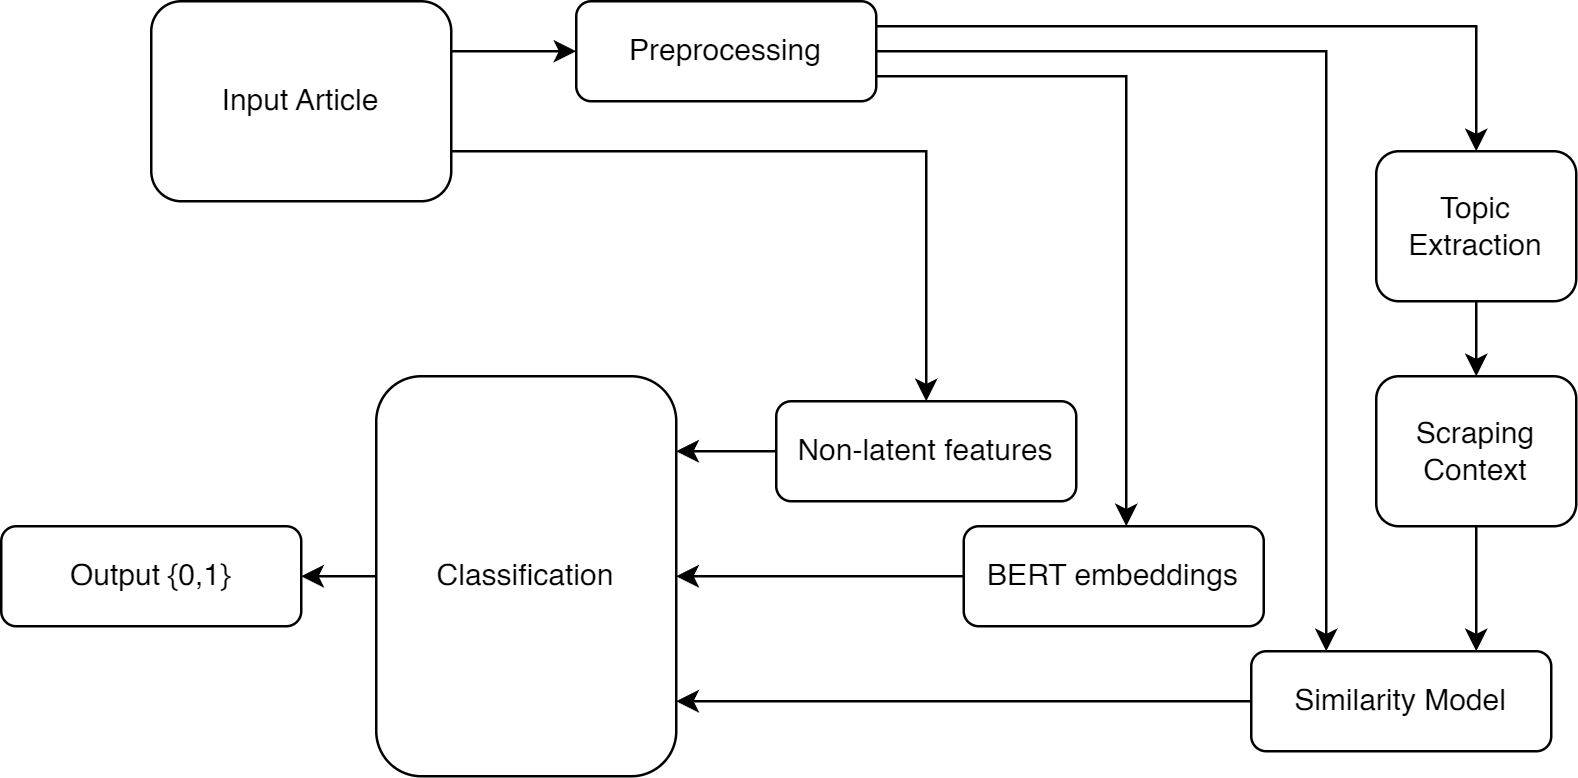
\includegraphics[width=0.6\textwidth]{img/pipeline.png}
    \caption{Our classification pipeline.}
    \label{pipeline}
  \end{wrapfigure}

  Figure~\ref{pipeline} shows our mostly linear classification pipeline. After preprocessing and tokenization, we extract contextual articles which are fed into a similarity model to form our first feature. Additionally, non-latent features from raw text and BERT embeddings form the rest of our features. The concatenation of all the features are fed into our classification models which infers a binary classification label.
\end{minipage}

\newsubsection{Preprocessing and tokenization}

\todojim{Write}

\newsubsection{Feature --- Similarity model}

One of the core aspects of our research was the ability to automatically gather articles that give some context to each input article. Our approach summarizes the input article so it can be used to find contextual articles. These articles can then be used for comparison to the input article.

\subsubsection*{Summary extraction}

To get the context articles, we need to summarize the main topic of our input article down to at most 10 keywords. We use the Python \verb|gensim|~\cite{py-gensim} library which provides various topic modelling interfaces for text inputs. We use the \verb|ldamodel| which implements Latent Dirichlet Allocation (LDA) to extract a single topic. LDA is a probabilistic model where the idea is you have a number of documents representing some latent topics characterized by a distribution over words. By feeding in the preprocessed sentences of our input article, we are able to get the main themes. We sort the output keywords by the probability they represent the topic then cap the amount of words to 10 at most.

For the scope of our research, we are able to perform manual validation of the summaries extracted to check the summary represented the article content well. Table~\ref{summary-extraction} shows some samples of items in our dataset after applying LDA. We see that while the summaries extracted are not perfect, they still represent the general meaning of the article. Two common issues we saw were:
\begin{itemize}
  \item Unordered words in the summary --- words representing the topics seemed to be unordered. To a human reading the summary by itself, they might be able to see that the words are all keywords of the article but put together in a sentence, will not completely make sense. We hypothesize that this could have caused sub-optimal results when we started scraping articles using the summaries.
  \item Appearance of stop words and other meaningless non-topic words in the summary --- As a flow on issue from our preprocessing, our summary was left with words such as ``wa'' (from ``was'') or ``ha'' (from ``has''). This would have impacted the meaning of our summary and later article scraping.\label{summary-extraction:bad-words}
\end{itemize}
We will discuss the possibility of extracting better summaries using a more robust model in Section~\ref{limitation:summary-extraction}.

\begin{table}
  \centering
  \begin{tabular}{cp{8cm}p{3cm}}
    \toprule
    ID & Article extract & Summary\\
    \midrule
    \verb|118_Real| & \articlecontent{118real}
    & email review fbi clinton said july comey news new wa\\
    \midrule
    \verb|15_fake| & \articlecontent{15fake}
    & home marines trump wa stickney way north plane family\\
    \bottomrule
  \end{tabular}
  \caption{Examples of summary extraction on items in dataset.}
  \label{summary-extraction}
\end{table}

\subsubsection*{Article scraping}

We feed the summary of the input article into Google News and collect the top three articles. We use Google News since it essentially provides a free PageRank algorithm which we can leverage to get the most popular articles during the time period. We will treat the articles we find as Real articles for purposes of comparison, i.e.\ an input article that is very different to our contextual article is likely to be Fake.

For our research, we will only manually feed in all summaries for our dataset. Our motivation for this research was to develop a tool that a user could potentially use to figure out if the current news they are reading contains misinformation. We acknowledge there exists APIs that provide either a wrapper around Google News or implement their own news search algorithm that we could have looked into. However, given the size of the dataset and our scope, this was not necessary to demonstrate our system.

\begin{quote}
  \textbf{SETUP:} We use a virtual machine with a freshly installed latest version of Google Chrome. Searches are condicted in ``Incognito Mode'' tabs. We also use a VPN to the West coast of the US. These invariants serve the main purpose so that Google's does not give any personalized results based on a browser fingerprint or IP address. We chose the US as the VPN destination since our dataset articles were extracted from US news sources and we wanted to scrape for articles with a similar style of writing. If you were to use the tool in Australia, Google would usually return articles from local sources. We restrict our scope to specifically this dataset rather than train on a wide dataset from all sources.

  Another invariant we implement is to add a \verb|before:2020| to our summary. This forces Google News to only find articles before this year so that the news we get won't be from recent news. A common discussion topic from our dataset was Donald Trump's 2016 election campaign and we know that the news regarding Trump in 2023 is much different to that of 2016. This makes sense as we are not using a very recent dataset so clamping the date we find contextual articles assumes that if were looking for fake articles at the time of reading the imput article, we wouldn't have too much future articles available.

  \textbf{PROCESS:} We attempt to get the top three articles and save the URL for each input article. Not all summaries returned three articles so we perform scraping in three passes:
  \begin{enumerate}
    \item We enter the whole summary without any changes. This is the most ideal approach and most machine-replicable. This covered 70\% of our dataset.
    \item Still performing only generic actions, we remove any~\hyperref[summary-extraction:bad-words]{\color{blue}bad words} or non-important connectives then searched again. This should still be machine-replicable with further work. This covered the next 20\% of our dataset.
    \item For the last 10\% of our dataset, we had to manually look at the input article content and summary generated to figure out why we still received no results. Our hypothesis was that this was a combination of our non-tuned summary extraction and the fact that some \emph{outrageous} Fake articles simply didn't have any similar articles that could be found. We will discuss this limitation in Section~\ref{limitation:article-scraping}.
  \end{enumerate}
  From the above passes, we were not able to find context articles for four input articles described in a table in Appendix~\ref{appendix:article-scraping}. Furthermore, we were only able to find one or two articles for some inputs but we can still continue with our similarity model.
\end{quote}

\begin{figure}[H]
  \centering
  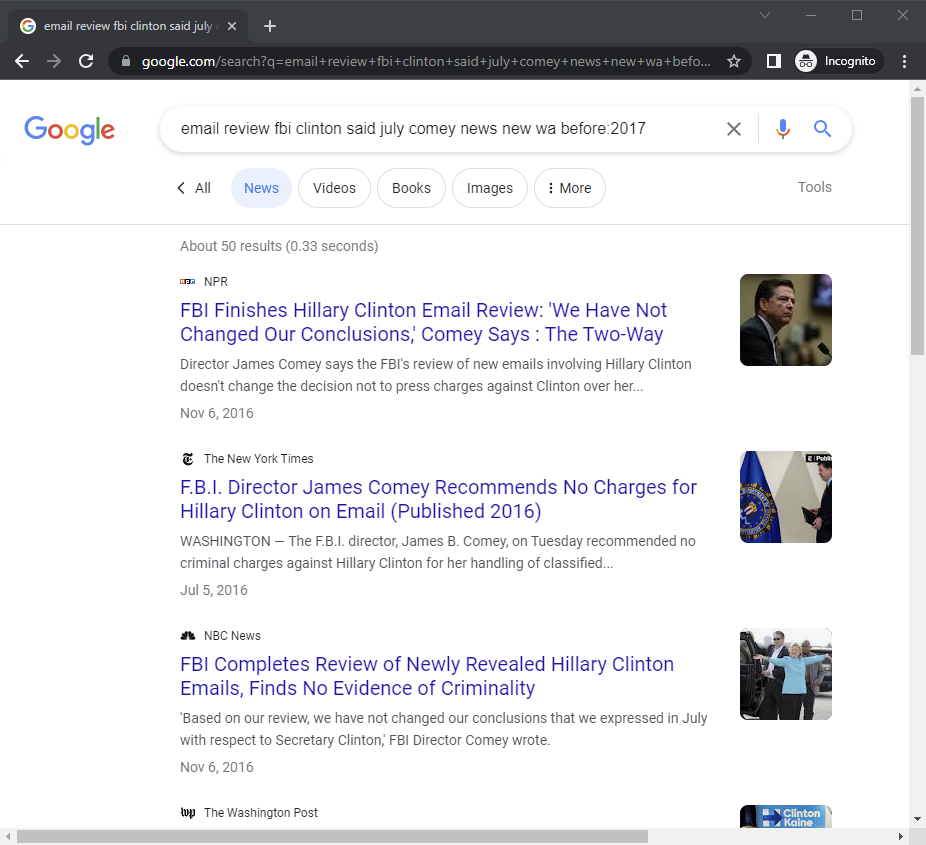
\includegraphics[width=0.4\textwidth]{img/chrome-article-scraping.png}
  \caption{Sample of articles found in Google after searching an article summary.}
\end{figure}

\noindent
After gathering three URL links for each context article, we use the Python \verb|newspaper3k|~\cite{py-newspaper} library to download the article and automatically extract its title and content.

\subsubsection*{Similarity model}

\tododuke{Write}

\newsubsection{Feature --- Non-latent features}

\tododuke{Write}

\newsubsection{Feature --- BERT embeddings}

\tododuke{Write}

\newsubsection{Model --- Machine learning}

\todojim{Write}

\newsubsection{Model --- Neural networks}

\tododhruv{Write}

\newsection{Experimental setup}

\newsubsection{Dataset}

\todojim{write}

\newsubsection{Evaluation metrics}

\todojim{write}

\newsection{Results and discussion}

\todojim{Machine learning}

\tododhruv{Neural nets}

\newsection{Conclusion}

\todoany{Summarise the study and discuss directions for future improvement}

\newsubsection{Limitations}

\todoany{Convert list of limitations to subsubsections with discussion.}

\begin{itemize}
  \item Summary extraction didn't produce perfect results~\label{limitation:summary-extraction}
  \item Article scraping sometimes returned no results even after manually figuring out why~\label{limitation:article-scraping}
  \item Models trained on only US news, may be a problem
\end{itemize}

\cleardoublepage
\pagebreak

\nocite{*}
\printbibliography

\cleardoublepage
\pagebreak

\appendix

\newsection{Individual contributions}

\begin{table}[H]
  \centering
  \begin{tabular}{lll}
    Jim & Dhruv & Duke \\
    \midrule
  \end{tabular}
\end{table}

\subsection{Jim}

\todojim{$\sim$1pg detailing individual contributions}

\subsection{Dhruv}

\tododhruv{$\sim$1pg detailing individual contributions}

\subsection{Duke}

\tododuke{$\sim$1pg detailing individual contributions}

\newsection{Article scraping}\label{appendix:article-scraping}

\begin{table}[H]
  \centering
  \begin{tabular}{cp{8cm}p{3cm}}
    \toprule
    ID & Article extract & Summary\\
    \midrule
    \verb|128_Real| & \small{\articlecontent{128real}} & god wa one never every king november still heart\\
    \midrule
    \verb|2_Fake| & \small{\articlecontent{2fake}} & ha adenugame africanamericans south femi united states africa president donald\\
    \midrule
    \verb|10_Fake| & \small{\articlecontent{10fake}} &wa room hotel maria told employee gonzalez hit video get\\
    \midrule
    \verb|34_Fake| & \small{\articlecontent{34fake}} &trump rage album machine band ha donald music outside year\\
    \bottomrule
  \end{tabular}
  \caption{Articles we were not able to find context articles for.}
\end{table}

\end{document}
